\documentclass[letterpaper, 12pt]{article}
\author{Nicola Corbellini}
\date{}
\title{Notes}


\usepackage[english]{babel}
\usepackage[margin=1in]{geometry}
\usepackage{amsmath}
\usepackage{xcolor}
\usepackage{bbm}
\usepackage{hyperref}
\usepackage{amssymb}
\usepackage[nottoc,numbib]{tocbibind}
\usepackage{amstext} 
\usepackage{eurosym}
\usepackage{float} 
\DeclareRobustCommand{\officialeuro}{%
  \ifmmode\expandafter\text\fi
  {\fontencoding{U}\fontfamily{eurosym}\selectfont e}}
  \usepackage{graphicx}
\usepackage{caption}
\usepackage{footnote}
\makesavenoteenv{table}
\makesavenoteenv{tabular}
\renewcommand{\baselinestretch}{1.25}



\begin{document}
\maketitle
\noindent

\subsection{Things TO DO (6-9-2025)}

\textbf{Writing.}
\begin{itemize}
    \item Paragraph on Adaptive Cluser Sampling (ACS) (Thompson, 1990, and Aga et al., 2022).
    \\ \textit{Thus far, the study of the informal sector has primarily come from household surveys, notably Labor Force Surveys, where questions on employment and income from the informal sector are added. While this approach provides valuable information, these are not surveys of businesses, and at best, they are a second-best approach to study informal business activity.
    \dots
    \\To study informal businesses, ACS is applied as follows. The geographic area of each covered city is divided into square blocks, each side 150 meters long. These blocks represent the primary sampling units. The methodology starts with a random selection of blocks, each of which is thoroughly enumerated. An enumerator canvasses the whole block and lists all informal businesses. Systematic listing captures information on the type of activity, physical location, and the number of workers, collected through an enumeration form. \dots In the process of enumeration, a sub-sample of informal businesses are randomly selected to conduct an interview.} (Aberra et al., Understanding Informality, Section 2.1)
    \item Definitions of informality: legal, fiscal, labor.
    \\\textit{A useful and basic typology of informality is the following: informality includes partial or full non-compliance with registration and licensing (legal informality), on employment (labor informality), or tax non- or under-payment (fiscal informality) (World Bank, 2020). This paper focuses on businesses’ activities that are legally informal: that is, lacking one or all of the registration or licensing requirements to operate. This definition must be anchored to the local context of implementation but generally consists of those businesses that lack a business license, do not exist on a business registry, and/or are not registered with the relevant tax authority.} (Aga et al., Surveying Informal Businesses)
\end{itemize}

\textbf{Data Work.}
\begin{itemize}
    \item Robustness checks: restrict analysis to cities and add micro data (formal less than 5) if available.
    \item 
\end{itemize}

\subsection*{WBES Informal (11/25/2024)}
Two types of WBES informal surveys:
\begin{itemize}
    \item \textbf{Earlier surveys} (before 2014, about 23 country-year): small samples, no weights, sometimes no uniform definition of variables, WB produced comprehensive database not available. Most (all?) informal surveys were implemented concurrently with standard WBES. However, lack of weights and representativeness makes it difficult to compute reliable shares of value added.
    \item \textbf{Most recent surveys} (after 2014, 14 country-year): larger samples, weights ensuring representativeness, WB produces comprehensive database available. 
    \begin{itemize}
        \item Roughly 37,000 observations
        \item Out of which 28,000 with information on sales
        \item Out of which 19,000 with information on wage bill and electricity.
        \item Minor differences in terms of sales between the 9,000 observations without wage bill the 18,000 with the wage bill.
    \end{itemize}
    \item \textbf{Most recent standard WBES surveys} (missing Somalia and Sudan, therefore 12 countries)
    \begin{itemize}
        \item Cleaned data so that they are harmonized with informal microdata
        \item About 18,000 observations (17,000 with sales and cost of employees)
        \item Two discrepancies with informal: city-region and weights
        \item Some work needed to match city from informal with city-region from standard. Easy in some cases, more difficult in others.
        \item \textcolor{red}{UPDATE Jan 2025: merged dataset WBES standard-micro-informal for 14 countries}
        \item If I exclude the observations from regions that are not in the informal data, I'll probably halve the size of the formal database. Not sure whether this is needed for representativeness; check documentation and other papers
        \item All the observations are weighted. But are weights comparable across standard and informal data? what are they representative of? check documentation and other papers. 
        \textcolor{red}{Update, Jan 2025: Contacted WBES by email, suggested comparability for employment and sales, not for value added. However, informality looks to be smaller than in the ILO data. Indian WBES data somewhat overrpresent micro formal.}
    \end{itemize}
    \item \textcolor{blue}{Aga et al.} (Surveying Informal Businesses: Methodology and Applications, 2022\footnote{See Section 2 of the paper about the shortcomings of labor foce surveys and enterprise surveys data.}) provide a useful distinction between three different concepts of informality:
    \begin{itemize}
        \item \textit{Legal informality}: partial or full non-compliance with registration and licensing.
        \item \textit{Labor informality}: partial or full non-compliance with employment.
        \item \textit{Fiscal informality}: partial or full non-compliance with tax payments.
    \end{itemize}
    This distinction is also represented in \textcolor{blue}{Medina and Schneider(2018)}, figure 3.1, based on \textcolor{blue}{Goymai and van de Ven (2014)}. Here legal informality is called \textit{economic underground}, while \textit{informal sector economy}, concerning registered production units, corresponds to fiscal and labor informality. Table 2 provides estimates for a small subset of countries using national statistics accounts.

    \item ILO definitions available at \href{https://ilostat.ilo.org/methods/concepts-and-definitions/description-labour-force-statistics/}{https://ilostat.ilo.org/methods/concepts-and-definitions/description-labour-force-statistics/}. 
    See also:
    \begin{itemize}
        \item \href{https://www.ilo.org/sites/default/files/wcmsp5/groups/public/@dgreports/@stat/documents/meetingdocument/wcms_894213.pdf}{https://www.ilo.org/sites/default/files/wcmsp5/groups/public/@dgreports/@stat/documents/meetingdocument/wcms\_894213.pdf}
        \item \href{https://www.ilo.org/sites/default/files/wcmsp5/groups/public/@dgreports/@stat/documents/normativeinstrument/wcms_901516.pdf}{https://www.ilo.org/sites/default/files/wcmsp5/groups/public/@dgreports/@stat/documents/normativeinstrument/wcms\_901516.pdf}
    \end{itemize}

    \item Employment outside the formal sector includes persons who are employed in the informal sector and in households, the latter of which is mainly comprised of persons employed by households as paid domestic workers. Employment in the informal sector refers to all the persons who, during a given reference period, were employed in at least one informal sector enterprise, irrespective of their status in employment and whether it was their main or a secondary job. (\textit{does this mean double counting? No, ``Statistics presented in ILOSTAT refer to the main job of employed persons, as the required information to assess (in)formality of the second job is usually not available.''})
    \\It must satisfy the following requirements:
    \begin{enumerate}
        \item \textit{Unincorporated market} enterprise.
        \item At least one of the following criteria:
        \begin{itemize}
            \item The number of persons engaged / employees / employees employed on a continuous basis, is below a threshold determined by the country (\textit{the size criterion does not appear in the chart though}. UPDATE: ``\textit{The harmonized series on informality are derived by the Department of Statistics from processing national household survey microdata files using a consistent navigational path. The process involves identifying the production unit (formal sector, informal sector or household) and the nature of the job (formal job or informal job) of each employed person in their main job in order to derive the final indicators.'' \textbf{Note that the path shown in the chart does not mention enterprise size.}} ).
            \item The enterprise is not registered.
            \item The employees of the enterprise are not registered.            
        \end{itemize}
    \end{enumerate}
    \noindent
    
    \item Note: Sampling weights are only available for formal enterprise surveys, because they are
    representative, and are used throughout the analysis. The weights are normalized so that they add
    up to 1 for each country. For informal firm surveys, sampling weights are not provided since they
    are not representative in the selected countries. Therefore, we assign a weight of 1 to each informal
    firm as commonly done in self-weighted surveys. The weights are normalized so that they add up
    to 1 for each country. Robust standard errors are reported for all our regressions.
    \href{https://www.enterprisesurveys.org/content/dam/enterprisesurveys/documents/research-1/Casting-a-Shadow-Productivity-of-Formal-Firms-and-Informality.pdf}{https://www.enterprisesurveys.org/content/dam/enterprisesurveys/documents/research-1/Casting-a-Shadow-Productivity-of-Formal-Firms-and-Informality.pdf}
    
    \item \textbf{TO DO LIST 11/25 - updated 11/27} \textcolor{red}{\textbf{ALL DONE JANUARY 2025}}:
    \begin{itemize}
        \item Check documentation. Check weights. Check other papers using microdata from BOTH standard and informal WBES (and MICRO!!!!).
        \item Harmonize city-region and weights to compute weighted value added.
        \item Is it possible to infer a share of informal value added from these data? How many assumptions are required?
    \end{itemize}

    \item \textbf{ETD data on employment}.
    Two primary sources of employment data exist, namely LFS data, which are collected at household level, and establishment surveys based on firm-level questionnaires. Both have their advantages and disadvantages for establishing annual sectoral employment trends.
    \\The LFS is a comprehensive and well-established source with substantive international harmonization of concepts because it uses definitions set out by the International Labor Organization (ILO), although sampling size and techniques differ between countries. The LFS aims to cover employees as well as the self-employed and family labour, although our investigation of sources suggests that in some surveys the self-employed and family labour are underreported in sectors that rely on this kind of worker. The main problem with LFS data is its limited consistency with output data from the NA, especially at the sectoral level, due the relatively small sample size. In addition, the sample is sometimes restricted to particular regions, such as urban areas, or is not properly stratified across regions or population subgroups.
    \\Information from establishment surveys (ES) is often more consistent with VA measures in the NA, because the output series for the NA are also based on this source. However, while the coverage by ES is reasonably accurate for goods-producing industries, this is not always the case for services. Moreover, ES typically cover only firms that surpass a certain threshold (for example, >20 employees or above a certain turnover level). This excludes smaller firms, which are especially abundant in developing countries. Another limitation is that data on self-employed and unpaid family members are usually not collected. This is problematic for sectors like agriculture and informal parts of the economy, where these categories make up a significant share of total employment. ES are therefore not well suited to the compilation of employment statistics by sector that cover the entire economy.
    \\Therefore, we normally use an alternative source based on household questionnaires but with a much more extensive coverage than the samples of the LFS: the population census (PC). This ensures full coverage of the working population and a reliable sectoral breakdown. However, PCs are typically quinquennial or decennial and cannot be used to derive annual trends.

    \item \textbf{Paper: Understanding Informality: Comprehensive Business-Level Data and Descriptive Findings}. There's a little bit on the representativeness of weights, but not on possible discrepancy between micro and informal WBES.

    \item \textbf{Document: Contextualizing informality: The Informal Economy Indicator Framework}.
    \begin{itemize}
        \item Employment indicators: aged 15 and older; 
        \item For employees in informal employment in formal economic units, to some extent for domestic workers in households and possibly for some dependent contractors, formalization calls primarily for the recognition and the declaration of the employment relationship and ensuring that effective access to social and labour protections is associated with it. For employees in informal employment in the informal sector, the formalization of the economic unit that employs them is also a precondition for the formalization of their job. \textcolor{red}{(This seems at odds with the fact that informal employment is lower than employment in the informal sector for some countries. I thought that the latter might be larger because there are formal workers in the informal sector. How can the latter be larger otherwise?)}
        \item Figure 6: informal employment prevalent in rural areas and in the agricultural sector, especially in lower-income countries.
    \end{itemize}

    \item Back to the figure

    % Figure
    \begin{figure}[H]
      \centering
      \caption{}
      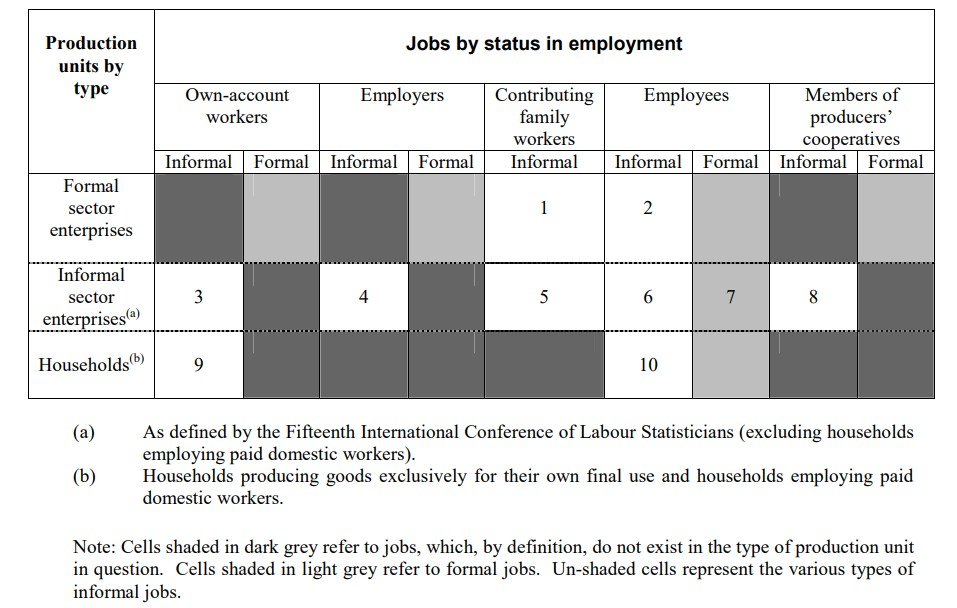
\includegraphics[scale=0.5]{informal_formal.jpg}
      \label{fig:my_label}
    \end{figure}

    If households cannot be identified, only the formal and informal sectors are tabulated. This occurs in many cases and as such, it is the rationale for deriving the final indicator on employment outside the formal sector, i.e. with the informal sector and households combined since these often cannot be differentiated.     
    \href{https://ilostat.ilo.org/methods/concepts-and-definitions/description-labour-force-statistics/#elementor-toc__heading-anchor-28}{ilo-website-link}


\end{itemize}



% % Figure
% \begin{figure}[H]
%     \centering
%     \caption{}
%     \includegraphics[scale=0.65]{}
%     \label{fig:my_label}
% \end{figure}


\end{document}

